%%%%%%%%%%%%%%%%%%%%%%%%%%%%%%%%%%%%%%%%%%%%%%%%%%%%%%%%%%%%%%%%%%%%%%%%%%%%%%%%
%%%%%%%%%%%%%%%%%%%%%%%%%%%%%%%%%%%%%%%%%%%%%%%%%%%%%%%%%%%%%%%%%%%%%%%%%%%%%%%%
%%%%%%%%%%%%%%%%%%%%%%%%%%%%%%%%%%%%%%%%%%%%%%%%%%%%%%%%%%%%%%%%%%%%%%%%%%%%%%%%
Este capítulo descreve com detalhes o ambiente de desenvolvimento que foi realizado neste projeto.

\section{Ambiente proposto}%

	O desenvolvimento do ambiente foi realizado para a plataforma web. Consiste em três partes principais:
	
	\begin{itemize}
		\item Editor de texto
		\item Montador
		\item Simulador
	\end{itemize}

	Toda a parte de interação com o usuário utiliza as tecnologias web: \textit{javascript}, para ter uma interface dinâmica, utilizando a biblioteca \textit{jQuery}. Para a estruturação utilizou-se a linguagem de marcação \textit{HTML}, e a folha de estilos \textit{CSS} para formatação do layout.

	Apesar de ter sido desenvolvido para rodar na web, os componentes "Montador" e "Simulador", podem ser utilizados separados, por exemplo em linha de comando. Basta ter instalado um interpretador \textit{Python 3.x}


\section{Arquitetura de software}

	Como na maioria das aplicações web, utilizamos o modelo Cliente-Servidor, como ilustrado anteriormente na figura \ref{fig:client-server-model}. Neste modelo, o usuário é um cliente, que faz requisições ao servidor através da internet. 

	Usuário faz requisição da página inicial, onde ele pode escrever seu código, então a partir disso ele irá enviar este código para o servidor, requisitando a montagem, e então receberá a saída do montador, ou a mensagem apropriada no caso de erros.

	Com o código montado, pode se salvar em arquivos os dados da montagem em diferentes formatos, binário, hexadecimal ou em formato \textit{MIF ("Memory Initialization File")}, utilizado para inicializar memórias em FPGA's da Altera. Esses dados podem ser enviados novamente para o servidor em uma nova requisição de simulação, e então o servidor irá responder os resultados do programa, qual o estado de memória final, valores dos registradores, e se houver, mensagens de saída.

	Para melhorar a interação do usuário com a ferramenta, foi utilizado a metodologia de \textit{Single Page Application}~\cite{mikowski2013single}. Desta maneira, utilizamos apenas uma página e carregamos conteúdos dinâmicamente na mesma página.

	Para a implementação da metodologia foi utilizado a biblioteca \textit{jQuery}. Existem tecnologias mais modernas mais apropriadas para a implementação de uma SPA, porém foi decido não utilizá-las por questões de tempo para a aprendizagem destas.

	O código \textit{jQuery} faz chamadas HTTP assíncronas ao backend usando os métodos POST e GET ao pressionar algum botão de ação do sistema. 

\section{Interface web}

	A interface web foi feita com as tecnologias padrões da web, HTML, CSS e Javascript. E faz parte do frontend da aplicação, onde o usuário irá interagir com a ferramenta. 

	Para a parte dinâmica do site foi utilizada a biblioteca jQuery, facilitando o desenvolvimento de funcionaliades no front-end principalmente na manipulação de elementos da tela. 

	Para o layout foi utilizado o framework Materialize CSS, com sua utilização perdemos menos tempo em detalhes de layout, e podemos focar mais nas funcionalidades.

	\begin{figure}[h]
	  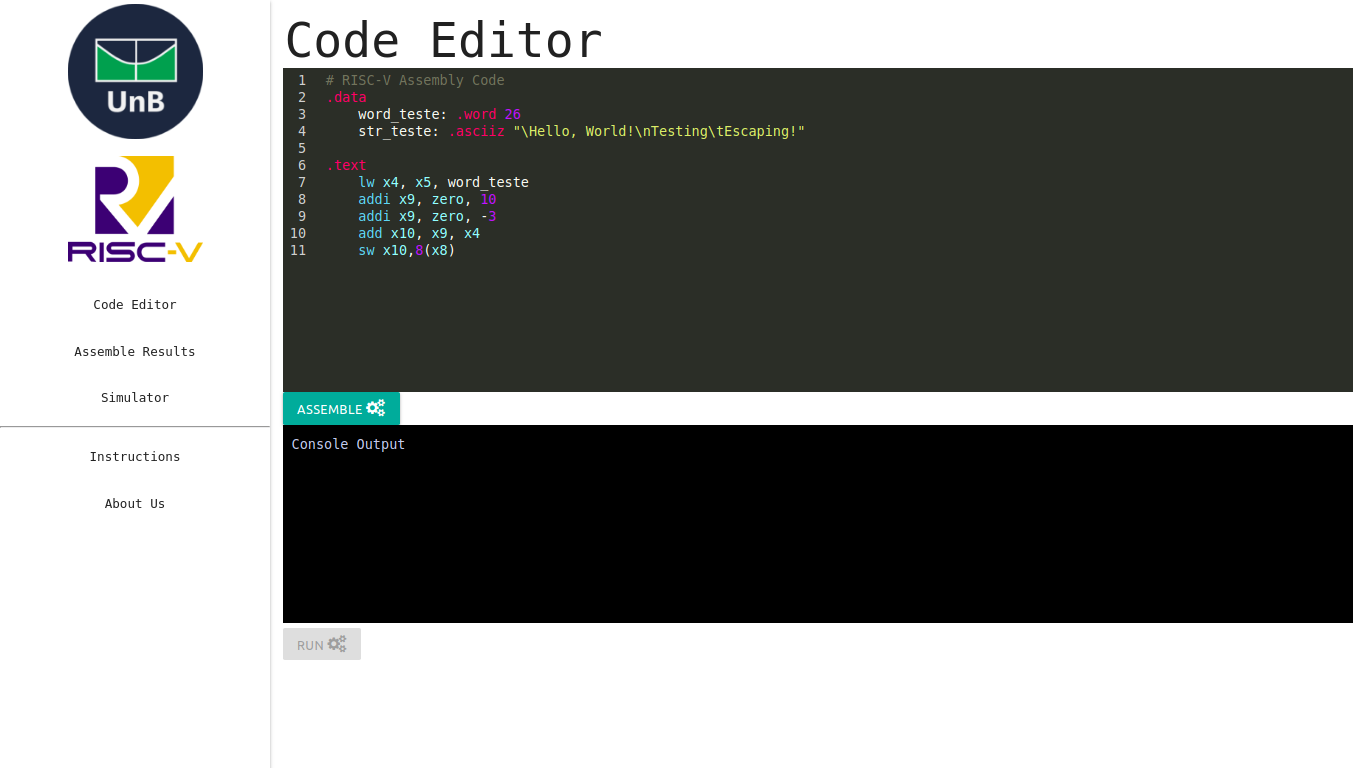
\includegraphics[width=\linewidth]{img/code_editor.png}
	  \caption{Página inicial, mostra o editor de texto com um código exemplo.}
	  \label{fig:editor_texto}
	\end{figure}

	Na figura ~\ref{fig:editor_texto}, vemos a tela inicial do sistema, a parte do editor de texto. No lado esquerdo da tela está o menu global, que está presente em todas as telas e serve para a navegação principal do sistema.

	Ao lado direito está o conteúdo da tela que consiste no editor de texto e um console de saída. O editor de texto utiliza a biblioteca open-source CodeMirror~\cite{codemirror}, escrita em javascript para criar editores de texto baseados em HTML.

	Após escrever o seu código, o usuário clica no botão \textit{ASSEMBLE}, se o montador não retornar nenhum erro não haverá mensagens no console e o botão \textit{RUN} será habilitado. Ao apertar o botão \textit{RUN} a tela irá ser trocaad para a tela de simulação, que mostraremos nas próximas seções.

	
\section{Montador}
	
	Utilizou-se neste projeto o algoritmo de duas passagens para montagem. Implementamos apenas as funcionalidades básicas para traduzir códigos \textit{assembly RISC-V} para código de máquina.

	O montador lida diretamente com a entrada do usuário, por isso essa parte pode ser considerada a mais crítica no projeto inteiro. Para que o sistema funcione corretamente a entrada do usuário, ou seja o código fonte, deve estar em um formato específico. E o sistema deve saber tratar os erros de acordo. 

	Alguns erros tratados no sistema como, símbolo inexistente, símbolo duplicado, erro de sintaxe, erro de tipo de argumento de instruções, número de argumentos da instrução, e alguns outros serão mostrados no próximo capítulo.

	Uma vez que o código foi montado com sucesso pode-se rodar através do botão \textit{RUN}, como dito anteriormente. Caso o usuário gostaria de utilizar o resultado da montagem em outro simulador, ou então exporar para uma \textit{FPGA}, se pode clicar no botão \textit{Assemble Results}, no menu global, do lado esquerdo da tela. e obter estes resultados. Exemplo pode ser visto na figura \ref{fig:assemble_data_bin}

	\begin{figure}[h]
	  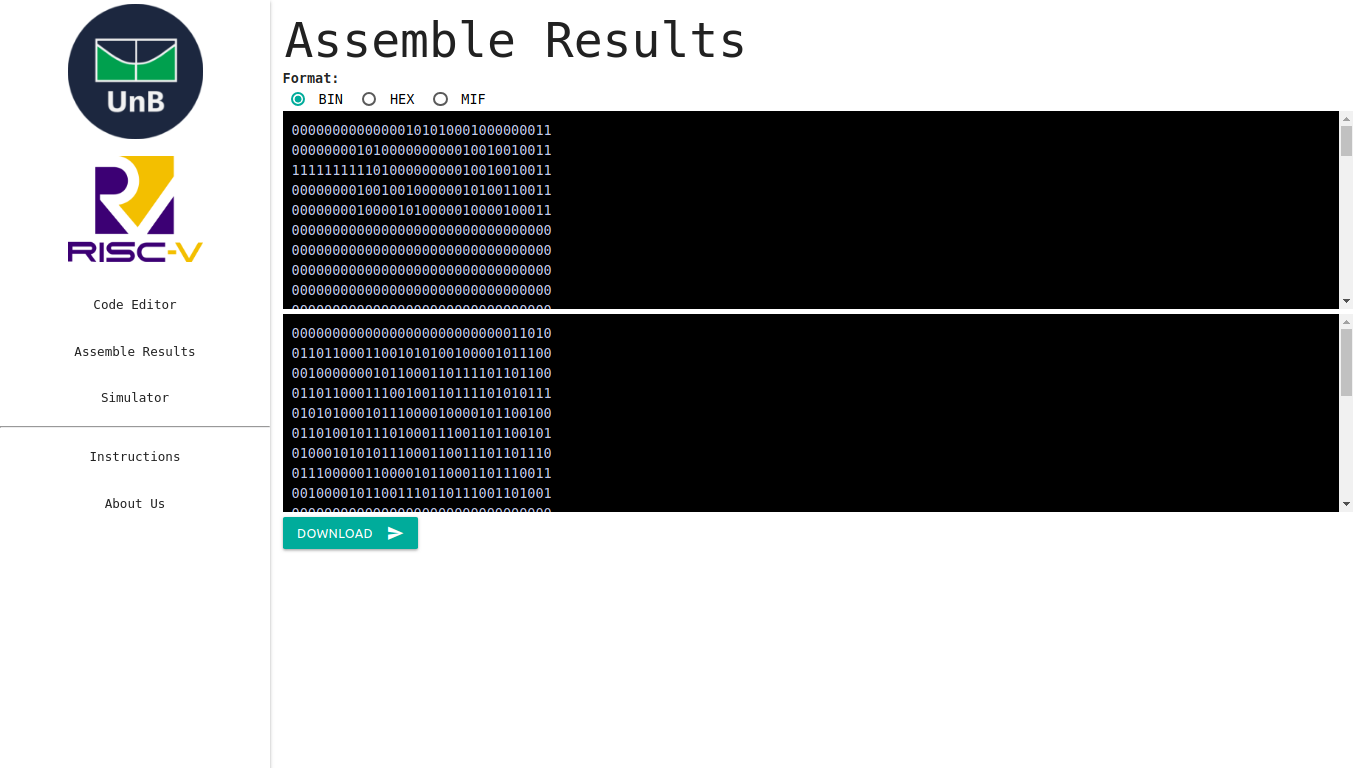
\includegraphics[width=\linewidth]{img/assemble_data_bin.png}
	  \caption{Resultados da montagem em binário.}
	  \label{fig:assemble_data_bin}
	\end{figure}

	Os resultados da montagem também podem ser visualizados em hexadecimal, ou formato MIF, como nas imagens \ref{fig:assemble_data_hex} e \ref{fig:assemble_data_mif}

	\begin{figure}[h]
	  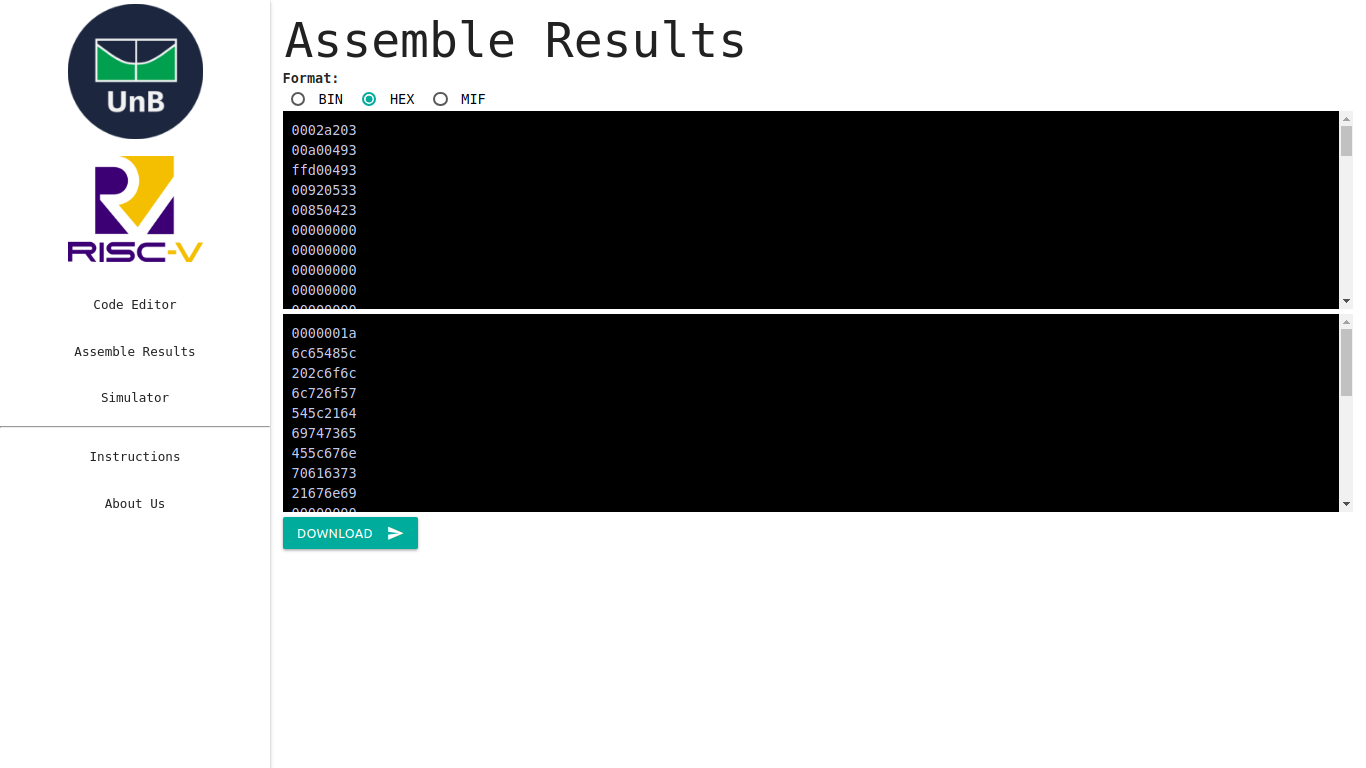
\includegraphics[width=\linewidth]{img/assemble_data_hex.png}
	  \caption{Resultados da montagem em hexadecimal.}
	  \label{fig:assemble_data_hex}
	\end{figure}

	\begin{figure}[h]
	  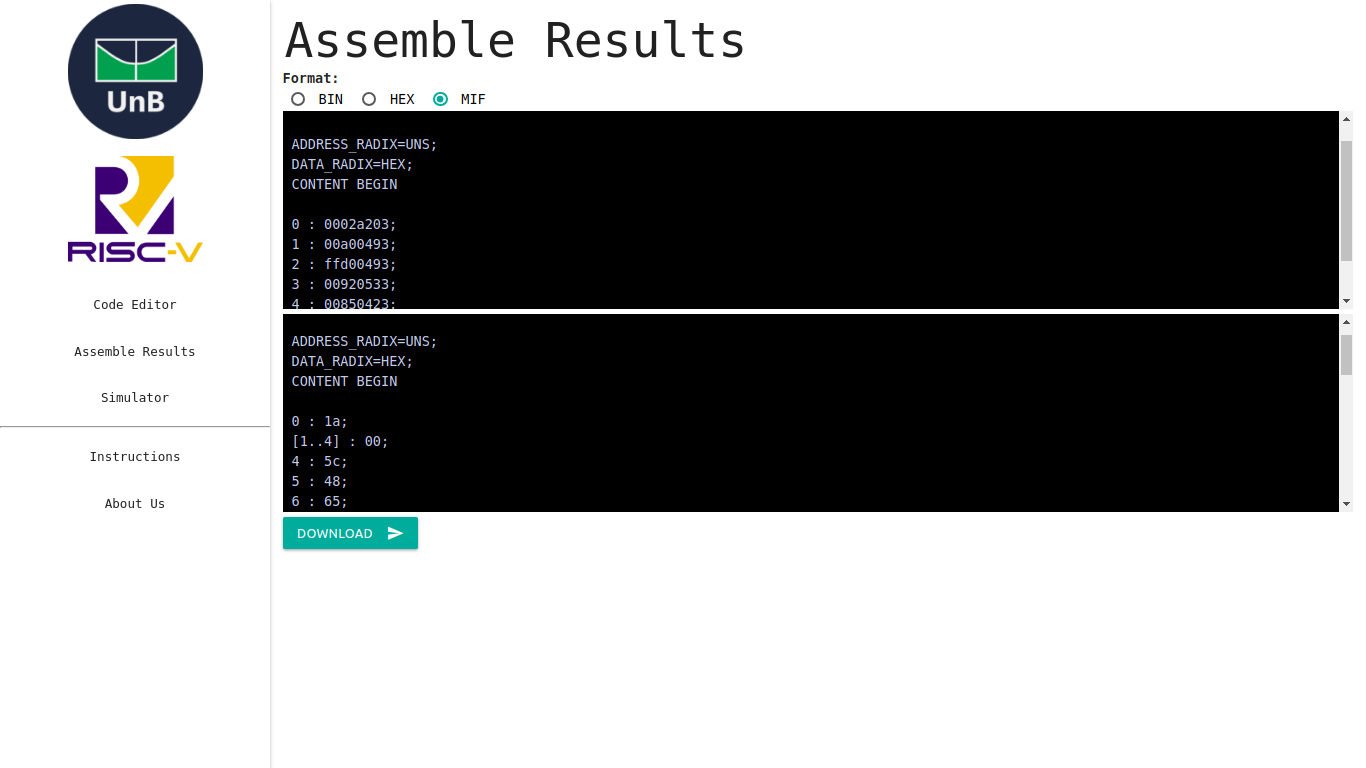
\includegraphics[width=\linewidth]{img/assemble_data_mif.png}
	  \caption{Resultados da montagem em formato MIF para FPGA.}
	  \label{fig:assemble_data_mif}
	\end{figure}



\section{Simulador}

	O simulador implementado neste projeto mostra o código montado, o código em hexadecimal, e as instruções que esses números em hexadecimal representam. Também pode se ver o mapa de memória e o estado dos registradores após o código montado ter sido executado ou em execução com a utilização do botão STEP.  Lembrando que foi implementado a arquitetura RV32G, portanto dispõe-se de 32 registradores de 32 bits.

	Na figura \ref{fig:simulator_results_1} é mostrado um exemplo dos resultados gerados pelo simulador implementado no projeto. O botão de RUN é utilizado para rodar o programa do momento em que está até o final da execução. Botão STEP irá executar apenas uma instrução. Pode-se utilizar o botão STEP para rodar algumas instruções e em seguida apertar RUN para executar até o final. A função de breakpoint não foi implementada. E o botão de RESET além de resetar as variáveis do sistema como os registradores, memória, program counter, também faz a montagem do código escrito na aba Code Editor.

	\begin{figure}[h!]
	  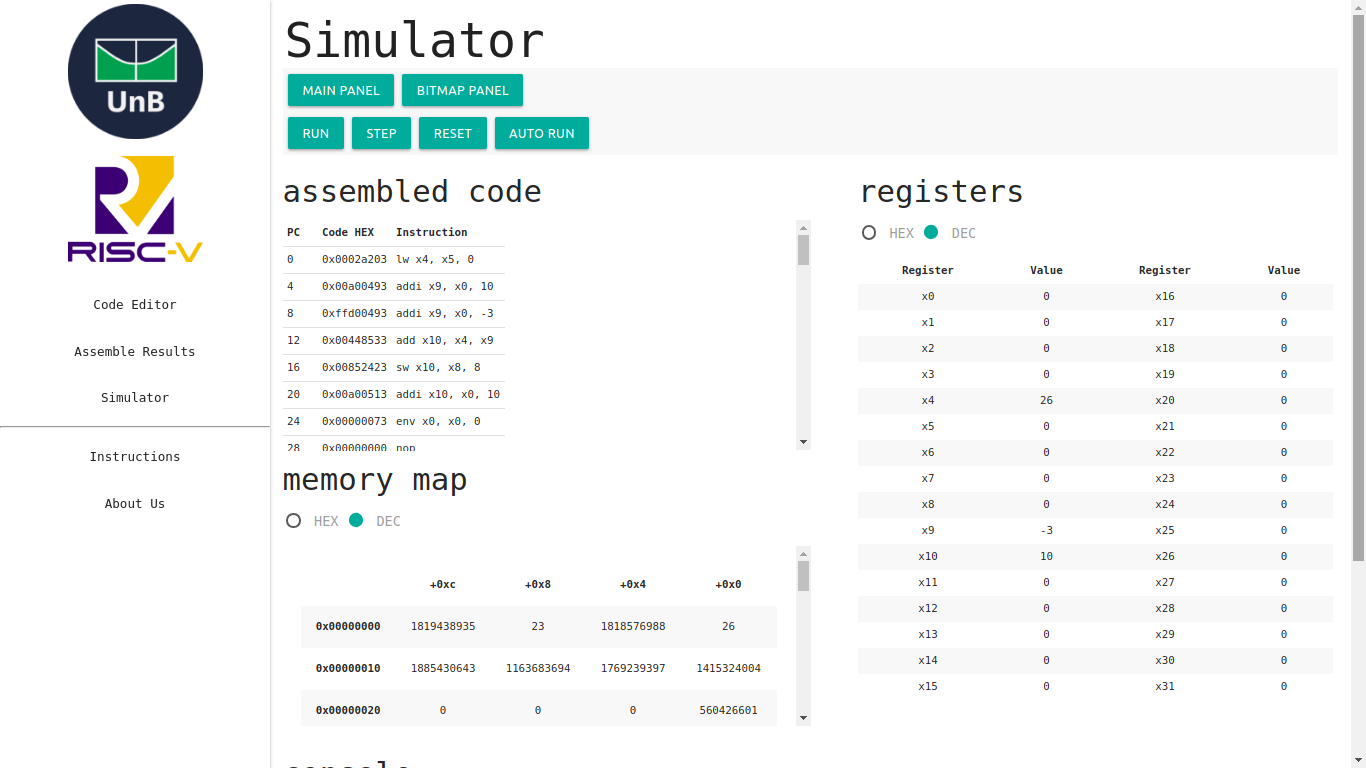
\includegraphics[width=\linewidth]{img/simulator_results_1.png}
	  \caption{Resultados do simulador. Código montado, mapa da memória, registradores. }
	  \label{fig:simulator_results_1}
	\end{figure}

	A figura \ref{fig:simulator_results_2} é a continuação da tela de resultados. Esta mostra uma tela de output do sistema. Neste projeto foi implementado apenas duas funções SYSCALL. Uma é a impressão de um inteiro, e a outra o encerramento do programa.  

	\begin{figure}[h!]
	  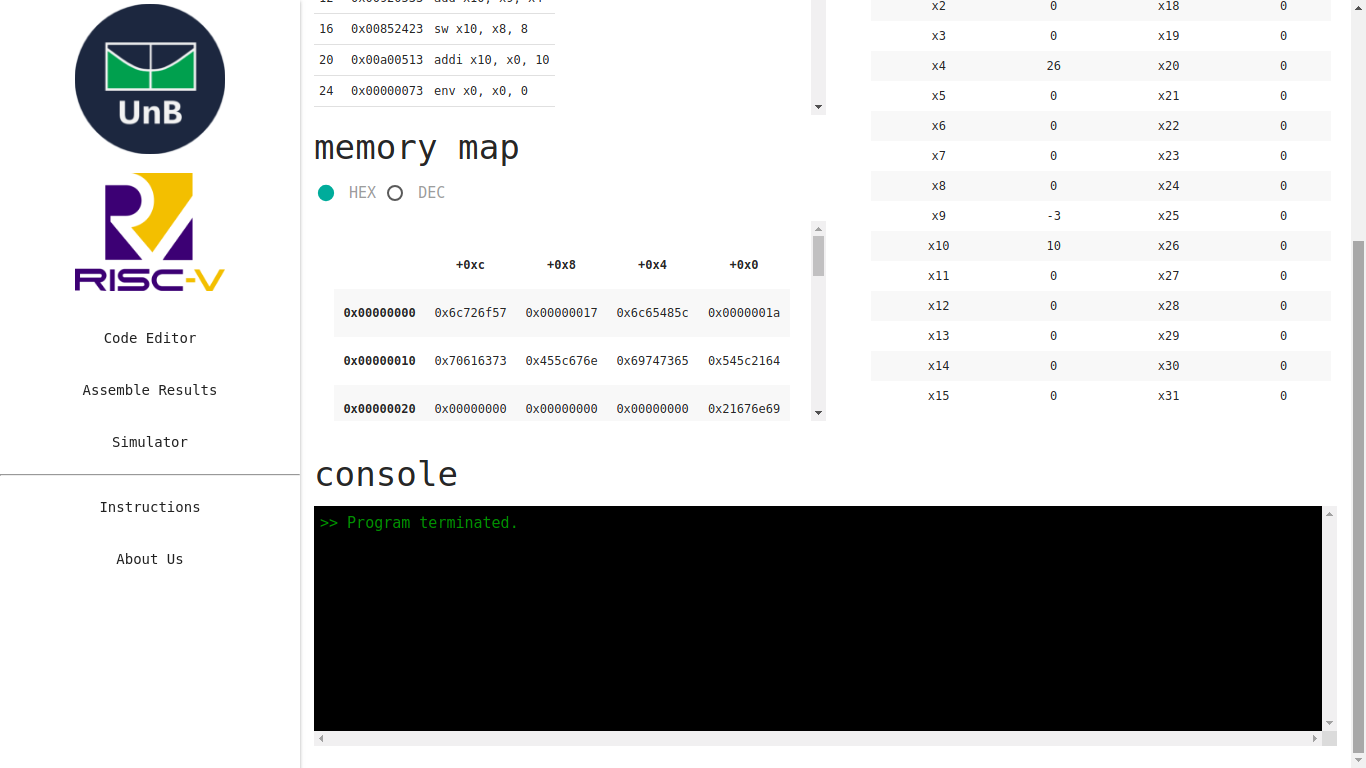
\includegraphics[width=\linewidth]{img/simulator_results_2.png}
	  \caption{Resultados do simulador. Console de saída de informações do sistema.}
	  \label{fig:simulator_results_2}
	\end{figure}

	Os valores de registradores e de mapa de memória podem ser visualizados na base decimal e hexadecimal.


\section{Extensiblidade}

	Este projeto tem como objetivo poder ser extendido por outros interessados no estudo da arquitetura. 

	Por exemplo, para casos onde se deseja performance, podem ser conectados modulos através de extensões para python como cython~\cite{cython_home}, a instalação automática desses módulos não pode ser feita nessa versão.
